\section{Introduction}
In this chapter, in section \ref{sec:crud} will be discussed the tests used to develop the two Kundera extensions.
IN section \ref{sec:performance} will be described the YCSB framework that we have used to test the performance of the developed extensions with respect to the low level API.
Finally in section \ref{sec:data} we present the application developed to test the data synchronization capabilities of CPIM while persisting data through the Datastore Kundera extension. 

\section{Test CRUD operations}
\label{sec:crud}
The Kundera extensions development, due to the lack of information both in the documentation and from the community, has been approached in a test driven way.
The first step was then writing the required JUnit tests for the features we have planned to support.

\newparagraph We primarily want to achieve code portability of model classes, this should be exploited by the usage of the JPA interface but, as stated in chapter \ref{chap:ps}, there were problems in the old NoSQL service implementation relatively to this point.
Secondary we want to be sure that while entities are persisted in the underlying NoSQL database, they can be restored without any loss of information and thus the mapping between entities and the NoSQL database data model behave correctly in both verses.
Hence test the extensions cannot be done directly by testing single methods behavior inside the extensions code, this will for sure test the correctness of the operations but, since Kundera clients are not obliged to follow a rigid structure for their code in the implementation of the required interfaces, tests written for a client are not guaranteed to run correctly for another one. 

\noindent The approach we adopted was to define a single test suite, that will test each one of the feature we planned to support, by interacting directly with Kundera through the JPA interface. This make us able to use the same tests independently of the specific extension and thus testing the correctness of CRUD operations through the JPA interface and the portability of the code by means of tests portability.

\noindent Those tests have been primarily used to test the extensions during the development phase but they have also been executed on the remote databases instances by connecting to them through the network from the development machine. This test has been made to guarantee the correct functioning of the two extensions on real databases instance since tests runned locally are executed  against emulators of real storages.

\subsection{Tests structure}
Tests are composed by the entities, annotated with the JPA annotations, and a test class for each feature.
There are 20 defined entities that includes:
\begin{itemize}
\item simple entities related with the JPA relationships annotations, used to test relationships among entities;
\item embeddable entities and specific entities that uses those embeddable entities as data types, both types used to test the embedded feature;
\item entities with enum fields, used to test the enum fields support;
\item entities declared with different data types for the primary key identifier, used to test ids auto-generation and user-defined ids validation.
\end{itemize}

\noindent The test classes developed for testing the correctness of relationships are:
\begin{itemize}
\item \texttt{MTMTest}, to test the \textit{Many to Many} relationship type;
\item \texttt{MTOTest}, to test the \textit{Many to One} relationship type;
\item \texttt{OTMTest}, to test the \textit{One to Many} relationship type;
\item \texttt{OTOTest}, to test the \textit{One to One} relationship type;
\end{itemize}
\noindent All of those test classes implements two different methods: \texttt{testCRUD()}, that test the relationship by interacting with the method of the \texttt{EntityManager} interface, and \texttt{testQuery()}, that test the relationships by reading, updating and deleting entities through JPQL queries.

\newparagraph The remaining tests classes are:
\begin{itemize}
\item \texttt{ElementCollectionTest}, that tests the JPA feature for persisting list of entities within another one;
\item \texttt{EmbeddedTest}, that tests the JPA feature of persisting user-defined data-types as field of entities;
\item \texttt{EnumeratedTest}, that tests the JPA feature of persisting enum fields;
\item \texttt{QueryTest}, that tests the execution of various \textit{SELECT} queries and the support for the various JPQL clauses in queries.
\end{itemize}

\section{Performance tests}
\label{sec:performance}

\subsection{Yahoo Cloud Serving Benchmark}
 
\subsection{YCSB adapters}

\subsection{YCSB tests results}

\section{Hegira generator}
\label{sec:data}
To be able to test the interaction between the CPIM library and the synchronization system and to provide an example of usage of the extended CPIM library, we have developed \textit{Hegira generator}.

\noindent The application provides two behaviors through command line interface, a \texttt{clean} command to clean-up the remote Datastore instance by deleting all the entities of all Kinds, and a \texttt{generate} command that take as argument the number of entities to be generated per table and generates them.

\newparagraph Data generation is done upon a pre-defined entity model inside the application and described by the ER diagram of figure \ref{fig:hegira-generator-er}.
Build an entity generator agnostic to the entities model was not our goal and it would have required a way to automatically build the dependency graph of the entities since entities related to other ones should have a reference to the entity they depends on. Hence the application is aware of the entities dependencies and generates them accordingly.

\begin{figure}[tbh]
  \centering
  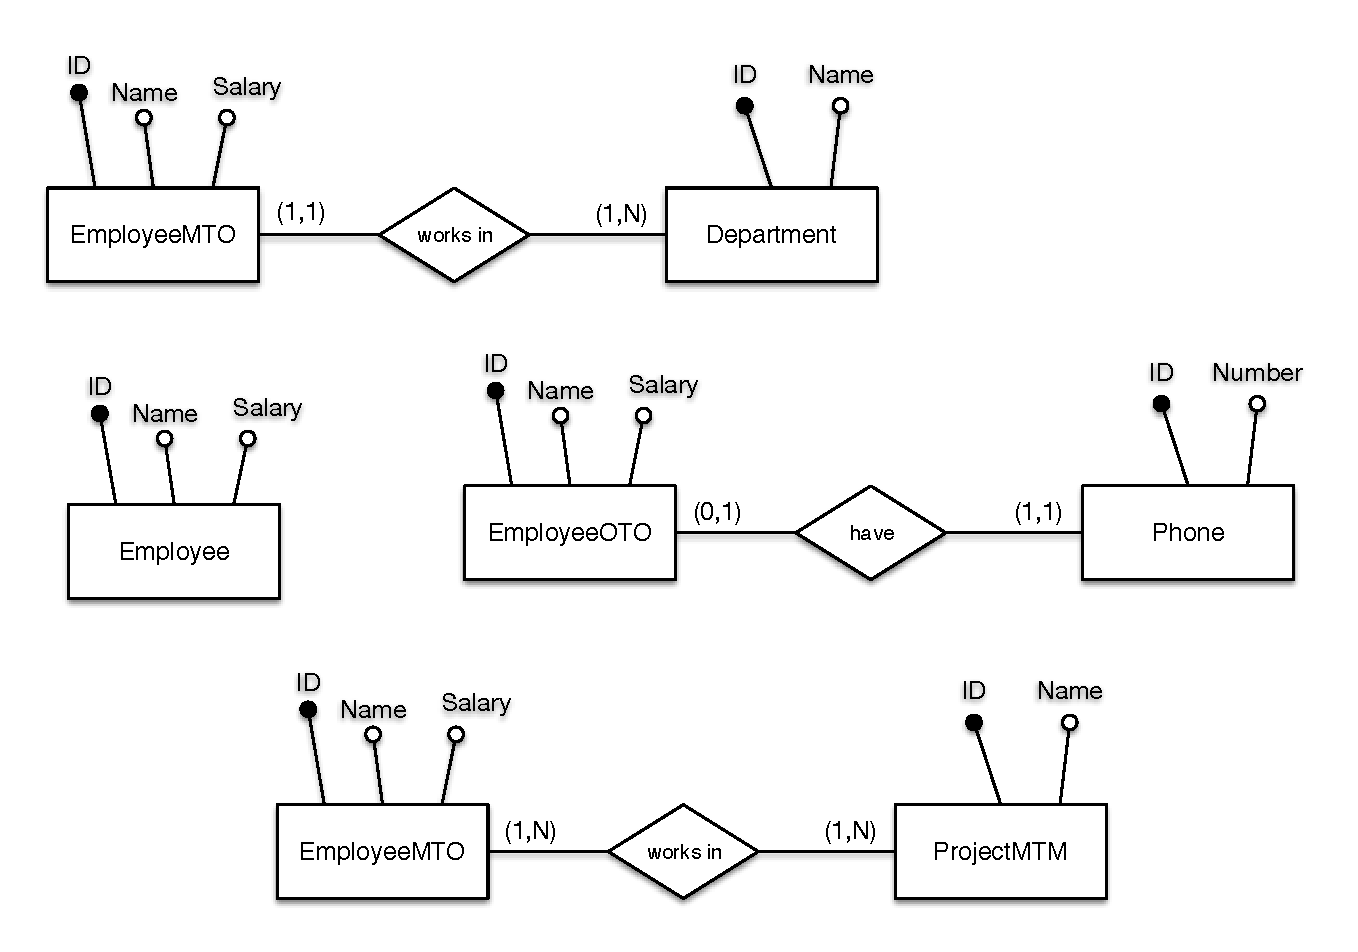
\includegraphics[width=10cm]{images/hegira_generator_er}
  \caption{ER diagram of Hegira-generator model}
  \label{fig:hegira-generator-er}
\end{figure} 

\noindent To be able to generate random entities, two methods are used:
\begin{itemize}
\item \texttt{persist(Class master)} that generates and persist entities without dependencies (such as \texttt{Employee} in the application model;
\item \texttt{persist(Class master, Class slave, DependencyType type)} that generates and persist the entities of the \textit{master} class, then uses randomly extracted entities among those just generated to fill the dependencies for the entities of the \textit{slave} class.
The \texttt{DependencyType} would be \texttt{SINGLE}, if the \textit{slave} class needs just one element to fill the dependency (which is the case of \textit{One to One} and \textit{Many to One} relationships), or \texttt{COLLECTION}, if the \textit{slave} class needs more than one element to fill the dependency (which is the case for \textit{Many to Many} relationships).
\end{itemize}

\noindent The actual entity generation is delegated to the entity itself through reflection since each entity of the model implements the \texttt{Randomizable} interface.
An example of entity genearion through this interface is shown in the snippet \ref{code:randomizable}.

\begin{lstlisting}[language=Java, caption=Entities generation, label=code:randomizable]
@Entity
public class EmployeeOTO implements Randomizable<EmployeeOTO, Phone> {
    ...
    @Override
    public EmployeeOTO randomize(Phone dependency) {
        setName(RandomUtils.randomString());
        setSalary(RandomUtils.randomLong());
        setPhone(dependency);
        return this;
    }
}
\end{lstlisting}
 
\subsection{Exploited CPIM features}
To perform the persist operation of the generated entities is used the \texttt{EntityManager} interface on which is called the \texttt{persist} method, this is completely JPA compliant and the user is not aware of what is done under the hood since communication with the synchronization system is handled automatically. An example is provided in the code \ref{code:example-persist}.

\begin{lstlisting}[language=Java, caption=Persisting entities in CPIM, label=code:example-persist]
CloudEntityManager em = MF.getFactory().getEntityManager();
Department dep = new Department("Computer Science")
em.persist(dep)
\end{lstlisting}

\noindent The persist operation through \texttt{CloudEntityManager} contacts the synchronization system to get the assigned sequence numbers for the specific tables and assign the first of them to the entity before delegating to Kundera the persist operation.

\newparagraph The application make use of the possibility of modifying at run-time the size of sequence numbers range that is requested to the synchronization system. Hence before the persist operation, the size of the sequence number range is set to the double of the number of entities to be generated. This is done through a call to \texttt{SeqNumberProvider.getInstance().setOffset(tableName, offset)}, if the resulting range size is grater than the maximum size that can be requested, is limited to that value. 

\newparagraph the last feature that is exploited by the application is the sequence number backup to file. The backup is configured in the \texttt{migration.xml} file as described in the appendix \ref{app:migration}.
This permit to the application, when is restarted, to restore the sequence numbers without the need of contacting the synchronization system.

\noindent Furthermore, to avoid execution of persist operations on a table which entities generation was completed in a previous execution, a file with the list of the table completely generated is kept in the same folder specified for the sequence numbers backup files.

\section{Summary}
In this chapter we have presented the test of correctness and performance made for the two developed Kundera extension showing the minimal performance loss that Kundera add to the low-level API.
Finally we have presented \textit{Hegira-generator}, the application developed to test the mechanisms developed inside CPIM to interacts with the synchronization system.
